\documentclass[aspectratio=169]{beamer}

%%%%%%%%%%%%%%%%%%%%%%%%%%%%%%%%%%%%%%%%%%%%%%%%%%%%%%%%%%%%%%%%%%%%%%%%%%%%%%%%%
% PREAMBLE

% DEFINE VARIABLES
\newcommand{\Lesson}{TEMA EJEMPLO}
\newcommand{\Subject}{Ejemplos, ejemplos, y ejemplos}
\newcommand{\Program}{Inversiones Financieras}
\newcommand{\Professor}{CUNEF Universidad}

% FOOTER WITH LOGO
\setbeamertemplate{footline}{
\hfill
\includegraphics[width=1.2cm]{figs/logo.png}\hspace{13cm}\vspace*{0.5cm}
\insertframenumber \hspace{1cm}
}

% FOOTER WITHOUT LOGO
\newcommand{\NoLogoFootline}{
    \setbeamertemplate{footline}{
    \hfill\vspace*{0.5cm}    
    }
}

% IDENTATION OPTIONS
\setlength{\leftmargini}{1em} % for itemize and enumerate level 1
\setlength{\leftmarginii}{1em} % for itemize and enumerate level 2
\setlength{\leftmarginiii}{1em} % for itemize and enumerate level 3

% PACKAGES
\usepackage[absolute,overlay]{textpos}
\usepackage{graphicx, tikz,xcolor}
\usepackage{multirow, bigstrut,epstopdf}
\usepackage{amsmath,relsize,bigdelim}
\usepackage{hyperref}
\hypersetup{
    colorlinks=true,
    linkcolor=blue,
    filecolor=magenta,      
    urlcolor=cyan,
}
\usepackage[font=tiny]{caption}

% COLOR OPTIONS
\definecolor{CUNEFOrange}{RGB}{255, 87, 0}
\definecolor{CUNEFGray}{RGB}{214, 209, 196}
\definecolor{Front}{RGB}{21,31,108}
% BEAMER OPTIONS
\setbeamertemplate{navigation symbols}{}
\setbeamercolor{itemize item}{fg = CUNEFOrange}
\setbeamercolor{itemize subitem}{fg = CUNEFOrange}
\setbeamercolor{itemize subsubitem}{fg = CUNEFOrange}		
\setbeamercolor{enumerate item}{fg = CUNEFOrange}
\setbeamercolor{enumerate subitem}{fg = CUNEFOrange}
\setbeamercolor{enumerate subsubitem}{fg = CUNEFOrange}		
\setbeamercolor{normal text}{fg=Front}

\setbeamercolor{frametitle}{fg=CUNEFOrange}


% NEW TITLE SLIDE
\newcommand{\CUNEFTitleSlide}{\begin{frame}

%\begin{textblock*}{0.1\paperwidth}(0.01\paperwidth,0.01\paperwidth)
%\includegraphics[width=0.3\paperwidth]{Logo_WQU.png}
%\end{textblock*}

\vspace{2em}
%\centering\scriptsize{{\textcolor{CUNEFOrange}{\Lesson}}} \\[1em]
\centering\textbf{{\large\textcolor{CUNEFOrange}{Econometrics 2024/2025}}} \\ [1em]
\centering{\large\textcolor{CUNEFOrange}{}} \\ [1em]
\vspace{0.5em}
\centering{\normalsize\textcolor{CUNEFOrange}{Multiple regression: additional aspects}}
\end{frame}}

% NEW SLIDE TEMPLATE
\newcommand{\slide}[2]{\begin{frame}
%\begin{textblock*}{0.1\paperwidth}(0.01\paperwidth,0.01\paperwidth)
%\includegraphics[width=0.15\paperwidth]{Logo_WQU.png}
%\end{textblock*}


\begin{textblock*}{0.87\paperwidth}(0.05\paperwidth,1.2cm)
{\Large\textcolor{CUNEFOrange}{#1}}
\end{textblock*}

\begin{textblock*}{0.87\paperwidth}(0.05\paperwidth,2cm)
#2
\end{textblock*}

\begin{textblock*}{\paperwidth}(0.01\paperwidth,0.95\paperheight)
\noindent\begin{tikzpicture}
%\draw[CUNEFOrange] (0,0) rectangle (0.9\paperwidth,0.8em);
%\draw[CUNEFOrange] (0.9\paperwidth+0.01\paperwidth,0) rectangle (\paperwidth-0.02\paperwidth,0.8em);
%\node[right] at (0,0.4em) {\tiny\textcolor{CUNEFGray}{\Subject\enspace-- \Program\enspace-- \Professor\enspace}};
\end{tikzpicture}
{\tiny\textcolor{CUNEFGray}\thepage}
\end{textblock*}
\end{frame}
}
%%%%%%%%%%%%%%%%%%%%%%%%%%%%%%%%%%%%%%%%%%%%%%%%%%%%%%%%%%%%%%%%%%%%%%%%%%%%%%%%%
% TOC AT BEGINNING OF EACH SECTION
\AtBeginSection[]{
    \begin{frame}<beamer>
    \frametitle{\textcolor{CUNEFOrange}{Outline}}
    \tableofcontents[currentsection]
    \end{frame}
}


\begin{document}

%%%%%%%%%%%%%%%%%%%%%
% Title Page
%%%%%%%%%%%%%%%%%%%%
\NoLogoFootline
{\usebackgroundtemplate{%
  
\includegraphics[width=\paperwidth,height=\paperheight]{figs/title_page.png}}
\CUNEFTitleSlide}


\setbeamertemplate{footline}{
\hfill
\includegraphics[width=1.2cm]{figs/logo.png}\hspace{13cm}\vspace*{0.5cm}
\insertframenumber \hspace{1cm}
}

\begin{frame}
\frametitle{\textcolor{CUNEFOrange}{Outline}}
   \tableofcontents 
\end{frame}


\section{More on Functional Form}
\frame<beamer>{\frametitle{\textcolor{CUNEFOrange}{Multiple Regression Analysis: Further Issues}}
More on Functional Form:
\begin{itemize}
\item More on using logarithmic functional forms: 
\item Convenient percentage/elasticity interpretation 
\item Slope coefficients of logged variables are invariant to rescalings  
\item Taking logs often eliminates/mitigates problems with outliers 
\item Taking logs often helps to secure normality and homoskedasticity  
\item Variables measured in units such as years should not be logged  
\item Variables measured in percentage points should also not be logged  
\item Logs must not be used if variables take on zero or negative values  
\item It is hard to reverse the log-operation when constructing predictions  
\end{itemize}
}

\frame<beamer>{\frametitle{\textcolor{CUNEFOrange}{Using quadratic functional forms }}

\begin{itemize}

    \item Example: Wage equation:
\begin{figure}
    \centering
    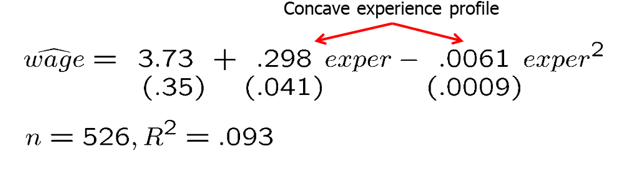
\includegraphics[width=0.6\linewidth]{figs/wage equation.png}
\end{figure}
    \item Marginal effect of experience 
\begin{figure}
    \centering
    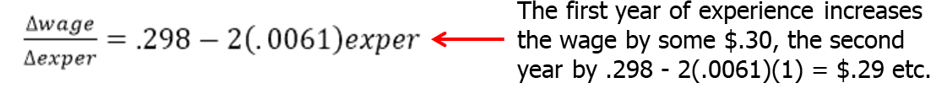
\includegraphics[width=0.85\linewidth]{figs/marg effect.png}
\end{figure}
\end{itemize}
}


\frame<beamer>{\frametitle{\textcolor{CUNEFOrange}{Wage maximum with respect to work experience}}
\noindent
\begin{minipage}{.45\textwidth}
   \begin{figure}[htp]
    %\centering
    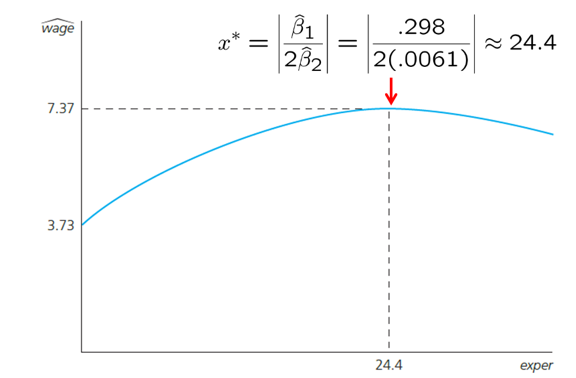
\includegraphics[width=1\textwidth]{figs/wage graph.png}
 \end{figure}
\end{minipage}%
\hspace{1cm} 
\begin{minipage}{.45\textwidth}
\begin{itemize}
    \item Does this mean the return to experience becomes negative after 24.4 years?

\item Not necessarily. It depends on how many observations in the sample lie to the right of the turnaround point.

\item In the given example, these are about 28\% of the observations. There may be a specification problem (e.g. omitted variables). 

\end{itemize} 

\end{minipage}
}

\frame<beamer>{\frametitle{\textcolor{CUNEFOrange}{Example: Effects of pollution on housing prices
}}


\begin{figure}
    \centering
    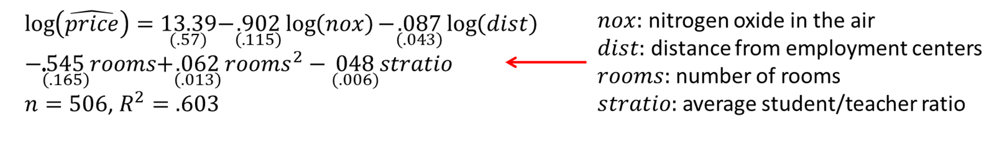
\includegraphics[width=1\linewidth]{figs/pollution.png}
\end{figure}
Does this mean that, at a low number of rooms, more rooms are associated with lower prices?
\begin{figure}
    \centering
    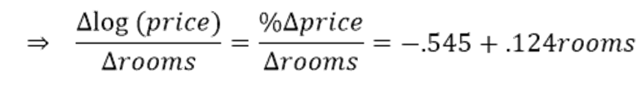
\includegraphics[width=0.7\linewidth]{figs/rooms.png}
\end{figure}

}


\frame<beamer>{\frametitle{\textcolor{CUNEFOrange}{Calculation of the turnaround point
}}
\centering

\begin{figure}
    \centering
    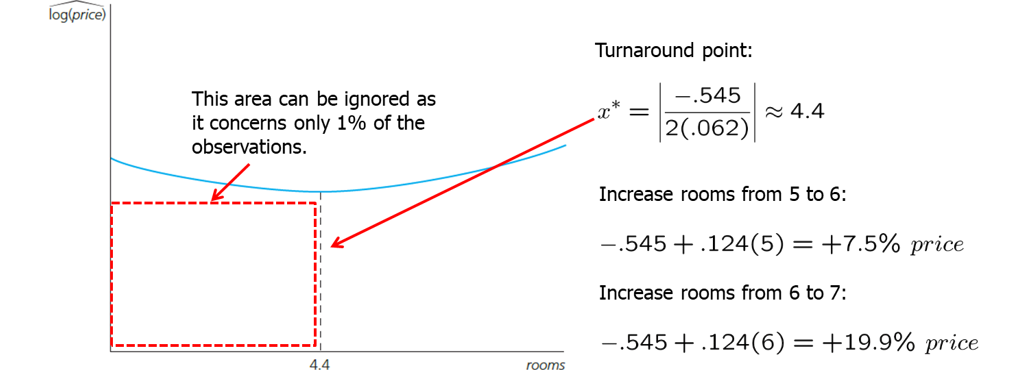
\includegraphics[width=1.1\linewidth]{figs/turnaround.png}
\end{figure}


}

\frame<beamer>{\frametitle{\textcolor{CUNEFOrange}{Other possibilities
}}
\begin{itemize}
\item Another model:
\begin{align*}
\text{log}(price) =& \beta_0 + \beta_1 \text{log}(nox) + \beta_2 [\text{log}(nox) ]^2 \\
&+ \beta_3 crime + \beta_4 rooms + \beta_5 rooms^2 + \beta_6 stratio + u
\end{align*}

$\Rightarrow  ~~~~~~ \frac{\Delta \text{log}(price)}{\Delta \text{log}(nox)} = \frac{\% \Delta price}{\% \Delta nox}= \beta_1 +2\beta_2 [\text{log}(nox) ]$
\end{itemize}
\hspace{1cm}
\begin{itemize}
\item Highter polinomials:
\begin{align*}
cost = \beta_0 + \beta_1 quantity + \beta_2 quantity^2 
+ \beta_3 quantity^3  + u
\end{align*}
\end{itemize}
}



\begin{frame}
    \frametitle{Models with interaction terms}
\begin{itemize}
\item Interaction term: sqrft *bdrms
    \begin{align*}
     price = \beta_0 + \beta_1 sqrft + \beta_2 bdrms + \beta_3  sqrft *bdrms + \beta_4 bthrms + u
    \end{align*}
\hspace{1cm}
$\Rightarrow \frac{\Delta price}{\Delta bdrms} = \beta_2 + \beta_3 sqrft$

\vspace{1cm}
\item Interaction effects complicate interpretation of parameters\\
$\beta_2 = $ Effect of bedrooms, but not for a square footage of zero
\end{itemize}
\end{frame}


\begin{frame}
    \frametitle{Reparametrization of interaction effects}
\begin{figure}
    \centering
    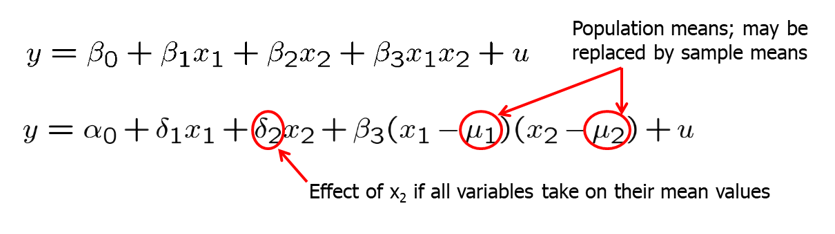
\includegraphics[width=1\linewidth]{figs/interact.png}
\end{figure}

Advantages of reparametrization:
    \begin{itemize}
        \item Easy interpretation of all parameters\medskip
        \item Standard errors for partial effects at the mean values available\medskip
        \item If necessary, interaction may be centered at other interesting values
    \end{itemize}
\end{frame}

\begin{frame}
    \frametitle{Average partial effects}
    \begin{itemize}
        \item In models with quadratics, interactions, and other nonlinear functional forms, the partial effect depend on the values of one or more explanatory variables
        \item Average partial effect (APE) is a summary measure to describe the relationship between dependent variable and each explanatory variable
	\item After computing the partial effect and plugging in the estimated parameters, average the partial effects for each unit across the sample
            \end{itemize}           
\end{frame}

\section{More on goodness-of-fit and selection of regressors}
\begin{frame}
    \frametitle{More on goodness-of-fit and selection of regressors}
General remarks on R-squared

    \begin{itemize}
        \item A high R-squared does not imply that there is a causal interpretation
\item A low R-squared does not preclude precise estimation of partial effects
\item Adjusted R-squared
\item What is the ordinary R-squared supposed to measure?
\item $R^2= 1- \frac{SSR}{SST} = 1-\frac{SSR/n}{SST/n}$ is an estimator for $1-\frac{\sigma^2_u}{\sigma^2_y}$ (population R-squared)
            \end{itemize}
            
\end{frame}


\begin{frame}
    \frametitle{Adjusted R-squared}
    \begin{itemize}
        \item A better estimate taking into account degrees of freedom would be
\[\bar R^2 = 1 - \frac{(SSR/(n-k-1))}{(SST/(n-1))} = adjusted ~ R^2
\]
\begin{itemize}
\item The adjusted R-squared imposes a penalty for adding new regressors
\item The adjusted R-squared increases if, and only if, the t-statistic of a newly added regressor is greater than one in absolute value

\end{itemize}
\item  Relationship between R-squared and adjusted R-squared
\[ \bar R^2 = 1 - (1- R^2)(n-1)/(n-k-1)\]
(The adjusted R-squared may even get negative!)
            \end{itemize}

          
\end{frame}


\begin{frame}
    \frametitle{Using adjusted R-squared to choose between nonnested models}
    \begin{itemize}
        \item Models are nonnested if neither model is a special case of the other

\[rdintens = \beta_0 + \beta_1 \text{log} (sales) + u
\]

$\rightarrow$ $R^2$ = .061, $\bar R^2 = .030$

\[rdintens = \beta_0 + \beta_1 sales + \beta_2 sales^2 + u
\]

$\rightarrow$ $R^2$ = .148, $\bar R^2 = .090$

\item  A comparison between the R-squared of both models would be unfair to the first model because the first model contains fewer parameters
\item In the given example, even after adjusting for the difference in degrees of freedom, the quadratic model is preferred
            \end{itemize}          
\end{frame}

\begin{frame}
    \frametitle{Comparing models with different dependent variables}
    \begin{itemize}
        \item R-squared or adjusted R-squared must not be used to compare models which differ in their definition of the dependent variable
	\item Example: CEO compensation and firm performance
	\begin{figure}
    \centering
    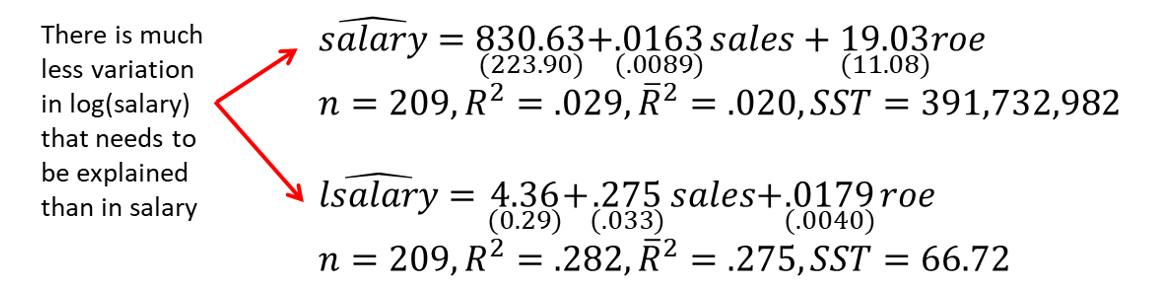
\includegraphics[width=1\linewidth]{figs/adjR.png}
\end{figure}
\end{itemize}          
\end{frame}

\begin{frame}
    \frametitle{Controlling for too many factors in regression analysis}
    \begin{itemize}
        \item In some cases, certain variables should not be held fixed
	\begin{itemize}
        \item In a regression of traffic fatalities on state beer taxes (and other factors) one should not directly control for beer consumption
	\item In a regression of family health expenditures on pesticide usage among farmers one should not control for doctor visits
	\end{itemize}  
\item Different regressions may serve different purposes

    \begin{itemize}
        \item In a regression of house prices on house characteristics, one would only include price assessments if the purpose of the regression is to study their validity; otherwise one would not include them

\end{itemize}
\end{itemize}          
\end{frame}

\begin{frame}
    \frametitle{Adding regressors to reduce the error variance}
    \begin{itemize}
        \item Adding regressors may excarcerbate multicollinearity problems
\item On the other hand, adding regressors reduces the error variance 
\item Variables that are uncorrelated with other regressors should be added because they reduce error variance without increasing multicollinearity
\item However, such uncorrelated variables may be hard to find
\item Example: Individual beer consumption and beer prices
\item Including individual characteristics in a regression of beer consumption on beer prices leads to more precise estimates of the price elasticity

\end{itemize}          
\end{frame}

\section{Prediction}
\begin{frame}
    \frametitle{Predicting when the dependent variable is logarithmic}
    \begin{itemize}
        \item Predicting $y$ when log$(y)$ is the dependent variable
\[
\text{log}(y)= \beta_0 + \beta_1 x_1 +\beta_2 x_2 + \ldots + \beta_k x_k +u
\]
$\Rightarrow y = \text{exp}(\beta_0 + \beta_1 x_1 +\beta_2 x_2 + \ldots + \beta_k x_k )\text{exp}(u)$

\item Under the additional assumption that $u$ is independent of $x_1,\ldots,x_k$:
\[\Rightarrow \text{E}(y|\mathbf{x}) =  \text{exp}(\beta_0 + \beta_1 x_1 +\beta_2 x_2 + \ldots + \beta_k x_k )\text{E}(\text{exp}(u))\]

\[\Rightarrow \hat y =  \text{exp}(\hat \beta_0 + \hat \beta_1 x_1 +\hat \beta_2 x_2 + \ldots + \hat \beta_k x_k )(\frac{1}{n}\sum_{i=1}^{n}\text{exp}(\hat u_i))\]
\end{itemize}          
\end{frame}

%%%%%%%%%%%%%%%%%%%%%
% Back Page
%%%%%%%%%%%%%%%%%%%%
\NoLogoFootline
{\usebackgroundtemplate{%

\includegraphics[width=\paperwidth,height=\paperheight]{figs/back_page.png}}
\slide{}{}}


\end{document}


